\documentclass{article}
\usepackage{graphicx}
\usepackage{url}
\usepackage{amssymb}
\usepackage{amsmath}
\usepackage{verbatim}
\usepackage{tikz}
\usepackage{rotating}
\usepackage{natbib}

\usetikzlibrary{positioning,petri}

%\SweaveOpts{width=6,height=4}

%\VignetteIndexEntry{Multiple table data in R}
%\VignettePackage{multitable}
%\VignetteDepends{multitable, MASS, lattice}
%\VignetteKeywords{data manipulation, ecology, multivariate, R}



\newcommand{\R}{{\sf R}}
\newcommand{\code}[1]{\texttt{#1}}
\title{Multiple-table data in \R}
\author{SC Walker}

\newcounter{exercise}
\numberwithin{exercise}{section}
\newcommand{\exnumber}{\addtocounter{exercise}{1} \theexercise \thinspace}

\usepackage{Sweave}
\begin{document}
\maketitle



\begin{abstract}
Data frames are integral to \R.  They provide a standard format for passing data to model-fitting and plotting functions.  This standard makes it easier for experienced use\R s to learn new functions, because most developments in \R\ continue to accept a single data frame as input.  Still, many data sets do not easily fit into a single data frame, and my field of community ecology provides many examples of such inherently multiple-table data (e.g. fourth-corner problem and other trait-based data sets).  Storing such data in a single data frame results in either large numbers of meaningless missing values or storage of redundant information.  These storage problems have led ecologists to model summaries of their data (e.g. community-weighted trait matrices), rather then their data itself.  Perhaps more importantly, my experience with manipulating such data using data frames has resulted in difficult-to-read workflows with many lines.  The \code{multitable} package introduces new data storage objects called \code{data.list}s, which are extensions of \code{data.frame}s.  As \code{data.list}s can be coerced to \code{data.frame}s, they can be used with all \R\ functions that accept an object that is coercible to a \code{data.frame} (e.g. \code{lm}; \code{plot}; \code{lme}; and many more).  The \code{multitable} package also provides several mechanisms for simplifying the manipulation of \code{data.list} objects.
\end{abstract}

\section{Introduction}

The standard data management paradigm in \R\ is based on \code{data.frame} objects, which are two-dimensional data tables with rows and columns representing replicates and variables respectively.  Standard \R\ workflows require that all of the data to be analyzed are organized into a single data frame, and hypotheses about the relationships between variables in the data frame are expressed using \code{formula} objects; data frames and formulas are combined by passing them to functions that produce analyses (e.g. plots; fitted models; summary statistics) \citep{ChambersAndHastie1992}.  This framework allows scientists to concentrate on their primary interests---the relationships between variables---without explicit reference to complex mathematical and algorithmic details.  It also provides access to those details, which are required (1) for more effective analyses and (2) to develop new methods of analysis within the framework.  As new methods are developed, researchers simply pass their data frames to new functions in much the same way they would pass them to older functions.  Thus, by separating low-level methods development from high-level data analysis, \R\ fosters the formation of a community of researchers where both methodologists and analysts can have mutually beneficial interactions.

However, research in my field of community ecology has led my colleagues and I to data sets that do not easily fit within a single data frame.  A common example is the fourth-corner problem \citep{LegendreEtAl1997}, in which three data tables are to be analyzed: a sites-by-species table of abundances or occurrences; a table of environmental variables at each site; and a table of traits for each species (Fig. \ref{fig:fourth}).  Such data are characterized by a conspicuous (lower-right) `fourth-corner', where there are no data.  These fourth-corners of missing data are not caused by the usual problems (e.g. broken field equipment; budget restrictions; bad weather; dead subjects), but are part of the study design itself.  The fourth-corner problem is a special case of a general `multiple-table problem', which can be much more complex (e.g. could involve three-dimensional `cubes' of data, Fig. \ref{fig:beatrix}).  The challenge of analyzing such multiple-table data sets in \R\ is that it is not obvious how to organize them into a single \code{data.frame}, which is required in standard \R\ workflows.  Our goal with the \code{multitable} package is to provide tools for analyzing multiple-table data sets within this standard \R\ framework.

\begin{figure}
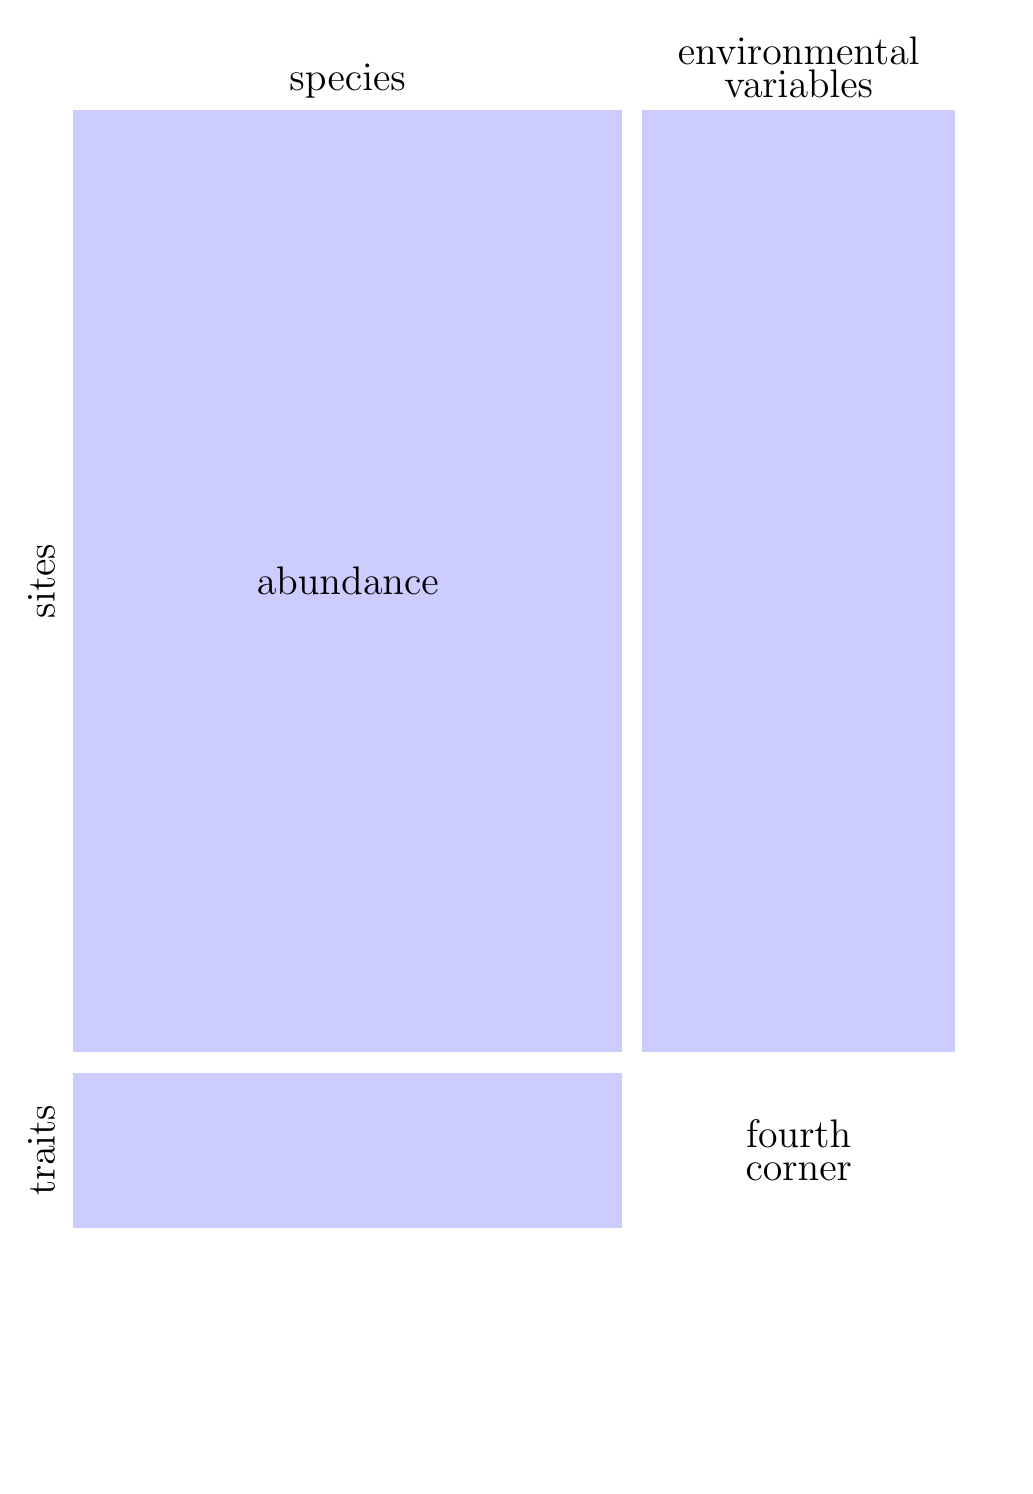
\begin{tikzpicture} [
	text centered,
	node distance=0.2cm,
	Y/.style={
		rectangle,draw=blue!0,fill=blue!20,thick,
		minimum width=7cm,minimum height=12cm,
		label=above:\Large species},
	X/.style={
		rectangle,draw=blue!0,fill=blue!20,thick,
		minimum width=4cm,minimum height=12cm,
		label={
		[text width=5cm]above:\Large environmental variables
		}},
	Z/.style={
		rectangle,draw=blue!0,fill=blue!20,thick,
		minimum width=7cm,minimum height=2cm},
	C/.style={
		rectangle,draw=red!0,fill=red!0,thick,
		minimum width=4cm,minimum height=2cm,
		text width=2cm},
	nm/.style={rectangle,minimum height=8cm,
	minimum width=0cm,draw opacity=0}
	]
\node [place,Y] 		(com)			{\Large abundance};
\node [place,X]	 	(env)[right=of com]	{};
\node [place,Z] 		(trt)[below=of com]	{};
\node [place,C]		(fc)[right=of trt]		{\Large fourth corner};
\node [place,nm]	(anm)[left=of com]	{\begin{turn}{90}
									\Large sites
								\end{turn}
								};
\node [place,nm]	(tnm)	[left=of trt]		{\begin{turn}{90}
									\Large traits
								\end{turn}
								};
\end{tikzpicture}
\caption{Fourth corner problem.} 
\label{fig:fourth}
\end{figure}

\begin{figure}
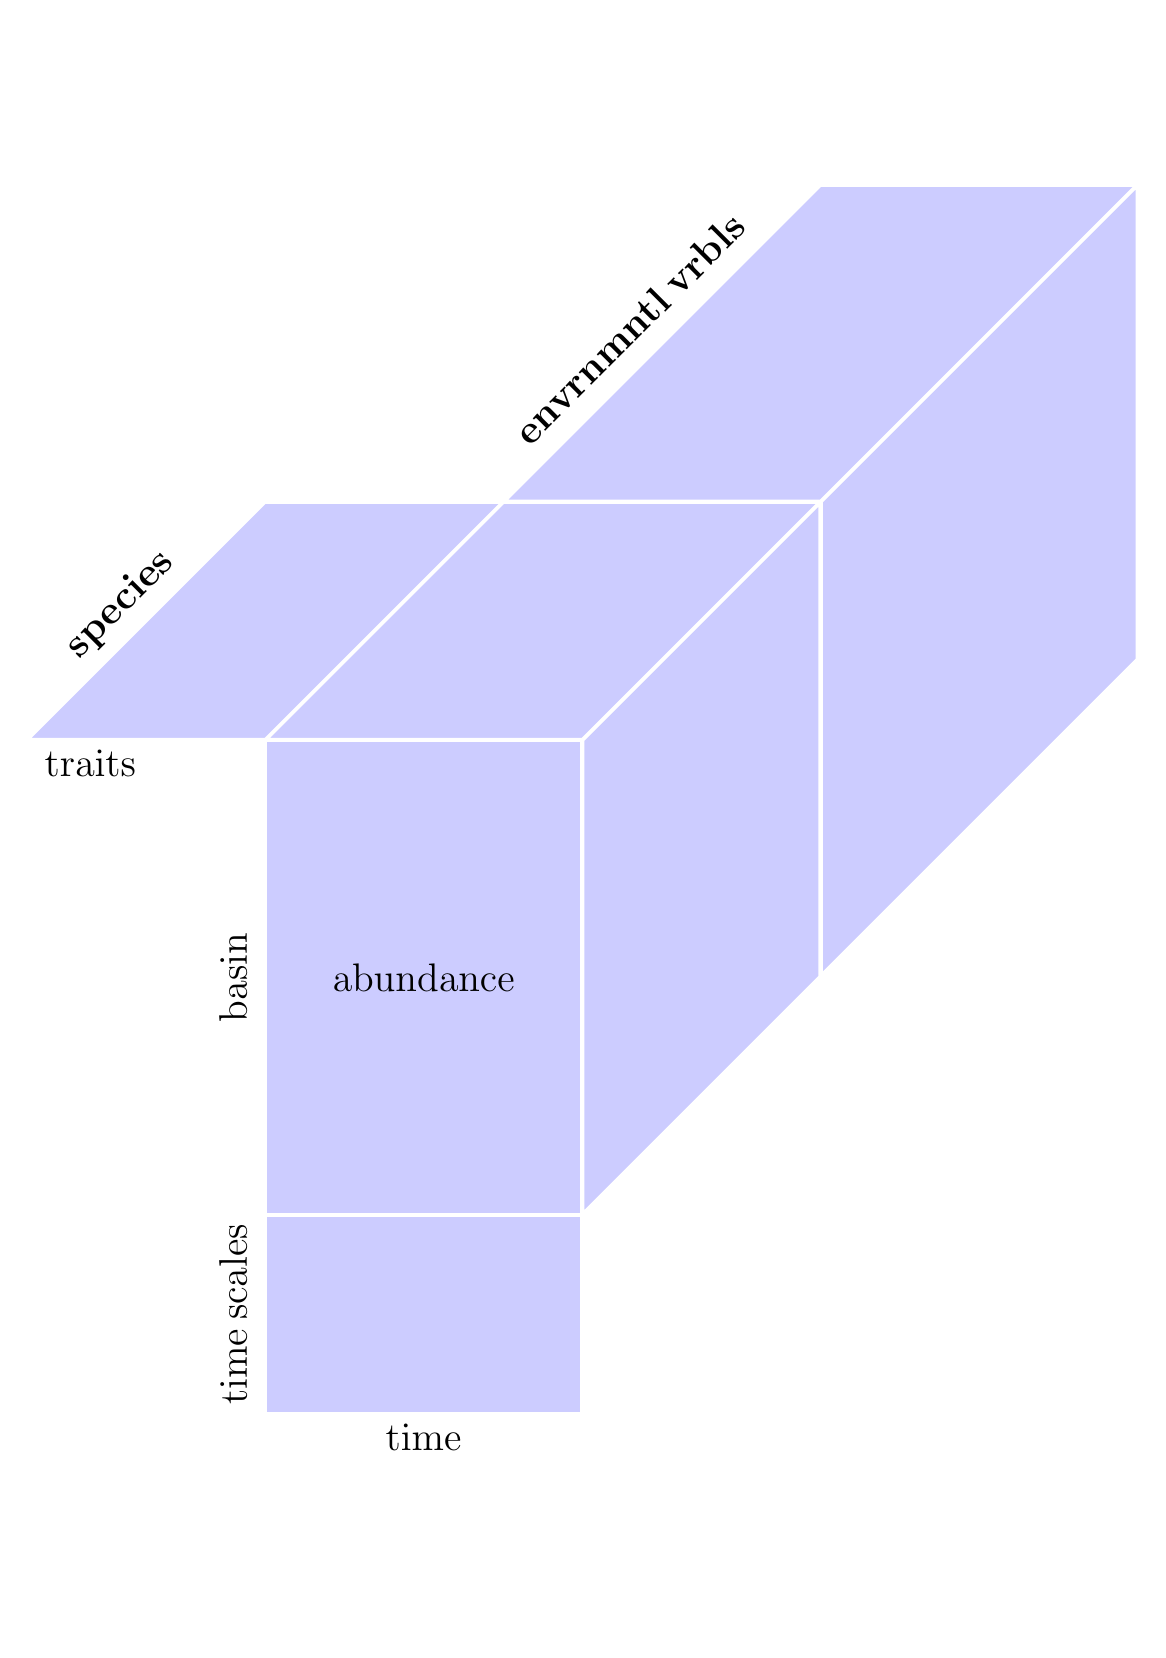
\begin{tikzpicture} [
	text centered,
	node distance=0cm,
	yfront/.style={
		rectangle,draw=blue!0,fill=blue!20,thick,
		minimum width=4cm,minimum height=6cm},
	time/.style={
		rectangle,draw=blue!0,fill=blue!20,thick,
		minimum width=4cm,minimum height=2.5cm,
		label=below:\Large time},
	ytop/.style={
		rectangle,draw=blue!0,fill=blue!20,thick,
		minimum width=4cm,minimum height=3cm,
		xslant=1},
	xtop/.style={
		rectangle,draw=blue!0,fill=blue!20,thick,
		minimum width=4cm,minimum height=4cm,
		xslant=1},
	yside/.style={
		rectangle,draw=blue!0,fill=blue!20,thick,
		minimum width=3cm,minimum height=6cm,
		yslant=1},
	xside/.style={
		rectangle,draw=blue!0,fill=blue!20,thick,
		minimum width=4cm,minimum height=6cm,
		yslant=1},
	trts/.style={
		rectangle,draw=blue!0,fill=blue!20,thick,
		minimum width=3cm,minimum height=3cm,
		xslant=1,label=below:\Large traits},
	frnm/.style={
		rectangle,minimum height=8cm,
		minimum width=0cm,draw opacity=0,
		text width=0.8cm},
	tpnm/.style={
		rectangle,minimum height=8cm,
		minimum width=0cm,draw opacity=0,
		xslant=0,text width=0.7cm}
	]
\node [place,yfront]		(front)			{\Large abundance};
\node [place,ytop]		(top)[above=of front]	{};
\node [place,yside]		(side)[right=of front]	{};
\node [place,trts]		(trts)[left=of top]	{};
\node [place,xtop]		(xtop)[above=of top]	{};
\node [place,xside]		(xside)[right=of side]	{};
\node [place,time]		(time)[below=of front]{};
\node [place,frnm]		(frnm)[left=of front]	{\begin{turn}{90}
										\Large basin
									\end{turn}
									};
\node [place,frnm]		(frnm)[left=of time]	{\begin{turn}{90}
										\Large time 
										scales
									\end{turn}
									};
\node [place,tpnm]		(tpnm)[left=of trts]	{\begin{rotate}{45}
										\hspace{-0.8cm}
										\Large
										\textbf{species}
									\end{rotate}
									};
\node [place,tpnm]		(tpnm)[left=of xtop]	{\begin{rotate}{45}
										\hspace{-2.1cm}
										\Large
										\textbf{
											envrnmntl 
											vrbls
										}
									\end{rotate}
									};
\end{tikzpicture}
\caption{The structure of the Lac Croche zooplankton community data.} 
\label{fig:beatrix}
\end{figure}

One possible solution is to develop new \R\ analysis functions---or new software packages altogether---that are specifically designed to accept several tables as input.  There has been a fair amount of work in this direction, focusing on data with a fourth-corner problem \citep{DoledecEtAl1996,LegendreEtAl1997,DrayAndLegendre2008,PillarEtAl2010,LeiboldEtAl2010,IvesAndHelmus2011}.  However, this work does not apply to data sets that have other more complex multiple-table data structures (e.g. zooplankton communities in Lac Croche, Fig. \ref{fig:beatrix}; Ref ??).  One approach to such issues would be to build new data analysis functions for each new data structure.  But such an approach is less than ideal, as it would require that new methods be learned for each new structure---it does not take advantage of the large number of tools developed within the standard \R\ framework of data frames and formulas.  The \code{multitable} package provides an alternative approach, by introducing a multiple-table generalization of data frames---called data lists---which can be analyzed with virtually any function that can be used to analyze a data frame.  Thus, instead of providing new methods of analysis, \code{multitable} provides new methods of data management.

There are several existing \R\ packages that are designed to make data management easier (e.g. \code{reshape2}; \citeauthor{Wickham2007}, \citeyear{Wickham2007}).  In fact, the \code{mefa} and \code{mefa4} packages have been developed to organize data with a slight generalization\footnote{Several community matrices---called segments---with identical dimensions are allowed in \code{mefa}.} of the fourth-corner problem \citep{Solymos2009}.  The \code{multitable} package has much in common with \code{mefa}, but there are noticeable differences.  For example, \code{mefa} provides more extensive tools for data summarization than \code{multitable} and \code{mefa4} integrates tools for sparse-matrix computations.  On the other hand, \code{multitable} is designed to handle more general data structures than \code{mefa} or \code{mefa4} (e.g. \code{mefa} cannot organize the Lac Croche data structure, Fig. \ref{fig:beatrix}).  However, we hope that \code{mefa} and \code{multitable} will be complementary, not competitive.

The \code{multitable} model of data organization is illustrated in Figure \ref{fig:model} (\code{mefa} uses a similar model).  The elements of the standard \R\ workflow are in blue: data frames; formulas; functions; and analyses.  The \code{multitable} package seeks to facilitate the use of such workflows with multiple-table data by creating tools (arrows and red boxes) for organizing and manipulating such data.  These tools are based on a new kind of object, called a data list, which is used to organize multiple-table data.  Data lists can be manipulated much like data frames (e.g. variables can be transformed; groups of observations extracted or removed).  Our design principle was to keep the manipulation of data lists as similar as possible to the manipulation of data frames.  Once data lists are ready for analysis \code{multitable} provides tools for coercing them into data frames, thereby entering the standard \R\ workflow.  Importantly, data, formulas, and functions are kept separate, thus preserving the benefits of using \R\ in this standard way.

\begin{figure}
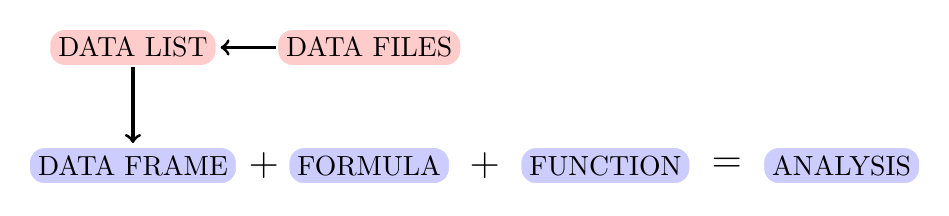
\begin{tikzpicture} [
	object stand/.style={
		rectangle,draw=blue!0,fill=blue!20,thick,
		rounded corners=2mm},
	object new/.style={
		rectangle,draw=red!0,fill=red!20,thick,
		rounded corners=2mm},
	otpt/.style={
		rectangle,draw=blue!0,fill=blue!20,thick,
		rounded corners=2mm},
	plus/.style={},
	tip/.style={
		->,shorten >=1pt,line width=0.4mm}]
\node[object new] (data files) 		at (3,1.5) {DATA FILES};
\node[object new] (data list) 		at (0,1.5) {DATA LIST};
\node[object stand] 	(data frame) 	at (0,0) {DATA FRAME};
\node[object stand] 	(formula) 		at (3,0) {FORMULA};
\node[object stand] 	(function) 		at (6,0) {FUNCTION};
\node[otpt]		(analysis) 		at (9,0) {ANALYSIS};
\node[plus] 					at (1.663,0) {\Large{+}};
\node[plus] 					at (4.47,0) {\Large{+}};
\node[plus] 					at (7.543,0) {\Large{=}};
\draw[tip] (data list.south) -- (data frame.north);
\draw[tip] (data files.west) -- (data list.east);
\end{tikzpicture}
\caption{The \code{multitable} paradigm for including multiple-table data (in red) into the standard \R\ workflow (in blue).  Data lists are used to organize and manipulate multiple-table data as a single \R\ object, even though it must be stored in multiple text-based data files.  When such data are required for analysis, they are coerced into a data frame.  Once in data frame form, they can be used in analyses by combining them with formulas (to specify hypothetical relationships between variables) and functions (to call computational methods).} 
\label{fig:model}
\end{figure}

The purpose of this vignette is to justify and introduce the use of the \code{multitable} package.  I begin by describing the structure of an example \code{data.list} object.  Then I illustrate one of the most powerful features of \code{data.list}s:  methods that allow related variables, which cannot fit into a single data frame, to be subscripted simultaneously.  Next I show that variables in data lists can be transformed and modeled, in the same manner that is standard for variables in data frames.  Finally, I describe a simple method for creating a data list of your own data, and use this method to introduce some useful concepts associated with multiple-table data.

\newpage
\section{The structure of data lists}

The \code{multitable} package comes with a fictitious \code{data.list}, to illustrate how these objects work.
\begin{Schunk}
\begin{Sinput}
> library(multitable)
> data(fake.community)
> fake.community
\end{Sinput}
\begin{Soutput}
abundance:
---------
, , capybara

            2009 2008 1537
midlatitude    4    0    0
subtropical    0   10    0
tropical       8    0    0
equatorial     0    7    0
arctic         0    0    0
subarctic      0    0    0

, , moss

            2009 2008 1537
midlatitude    0    6    0
subtropical    0    0    0
tropical       9    0    0
equatorial     0    3    0
arctic         5    0    0
subarctic      0    0    0

, , vampire

            2009 2008 1537
midlatitude    0    0    0
subtropical    0    0    1
tropical       0    0    0
equatorial     0    0    0
arctic         0    0    0
subarctic      0    0    0

Replicated along:  || sites || years || species || 


temperature:
-----------
            2009 2008 1537
midlatitude   NA   10   NA
subtropical   25   20   NA
tropical      48   50   NA
equatorial    50   30   NA
arctic       -37  -30   NA
subarctic      3    0   NA
Replicated along:  || sites || years || 


precipitation:
-------------
            2009 2008 1537
midlatitude   NA   20   NA
subtropical   99  100   NA
tropical     149  150   NA
equatorial   199  200   NA
arctic        21   20   NA
subarctic     41   40   NA
Replicated along:  || sites || years || 


body.size:
---------
capybara     moss  vampire 
     140       NA      190 
Replicated along:  || species || 


metabolic.rate:
--------------
capybara     moss  vampire 
      20        5        0 
Replicated along:  || species || 


homeotherm:
----------
capybara     moss  vampire 
       Y        N        N 
Levels: N Y
Replicated along:  || species || 


REPLICATION DIMENSIONS: 
  sites   years species 
      6       3       3 
\end{Soutput}
\end{Schunk}

At first sight, this \code{data.list} object looks very different from standard \code{data.frame} objects, but on second look we can see that they are really quite similar.  Just like data frames, data lists are composed of a number of variables---in this case, we have six variables (abundance; temperature; precipitation; body size; metabolic rate; and homeotherm) each identified in the printed object above by underlined names.  The variables in data lists must be printed in this sequential manner, rather than as columns neatly lined up in a data frame, precisely because the variables in multiple-table data sets do not line up neatly; this is the problem \code{multitable} seeks to address.

Also as in data frames, the replication of variables in data lists are represented as vectors of values.  The main difference between the two objects in this regard is that the vectors that represent variables in data lists have a \code{dim} (i.e. dimension) attribute, which gives it further structure.  In \R, vectors with \code{dim} attributes are best thought of as matrices and arrays of numbers.  For example, the \code{abundance} variable is replicated along three dimensions (sites; years; and species), and therefore is a three dimensional array of data.  This information is indicated above after the variable itself is printed.  Some variables are only replicated along two dimensions (e.g. temperature and precipitation) and others only a single dimension (e.g. body size; metabolic rate; and homeotherm).  

Importantly however, although the variables are not replicated along all of the same dimensions, they do share dimensions; and it is this dimension sharing that allows us to relate variables to each other.  To appreciate the dimension sharing of this example, we can use the \code{summary} method for \code{data.list} objects.
\begin{Schunk}
\begin{Sinput}
> summary(fake.community)
\end{Sinput}
\begin{Soutput}
        abundance temperature precipitation body.size
sites        TRUE        TRUE          TRUE     FALSE
years        TRUE        TRUE          TRUE     FALSE
species      TRUE       FALSE         FALSE      TRUE
        metabolic.rate homeotherm
sites            FALSE      FALSE
years            FALSE      FALSE
species           TRUE       TRUE
\end{Soutput}
\end{Schunk}
\noindent This method returns a logical table with dimensions of replication as rows and variables as columns.  A value of \code{TRUE} appears in cells corresponding to variables that are replicated along a particular dimension, and a value of \code{FALSE} appears otherwise.  We can see that the \code{sites} and \code{years} dimensions relate \code{abundance}, \code{temperature}, and \code{precipitation}; whereas, the \code{species} dimension relates \code{abundance}, \code{body size}, \code{metabolic rate}, and \code{homeotherm}.

Note that some \code{FALSE} entries are bio-physical necessities, whereas some are properties of the study design.  For example, suppose that later in the study, the researchers decided that it was necessary to get some idea of the spatial variation in metabolic rates.  It would then be possible to measure metabolic rates of the species at different sites, thereby changing the \code{FALSE} associated with the metabolic rate-sites cell to a \code{TRUE}.  To the contrary, it is physically and logically impossible to measure the precipitation of a species, and so this \code{FALSE} is necessarily \code{FALSE}.

\section{Subscripting data lists}

This structure relating variables and dimensions of replication, allows us to manipulate multiple variables simultaneously.  In particular, \code{multitable} makes it possible to extract pieces of a data list while maintaining its structure.  For example, examining the data suggests that 1537 might have been an outlying year relative to 2008 and 2009.  We can exclude data from 1537 just as we would with a single \R\ array.
\begin{Schunk}
\begin{Sinput}
> fake.community[,c("2008","2009"),]
\end{Sinput}
\begin{Soutput}
abundance:
---------
, , capybara

            2008 2009
midlatitude    0    4
subtropical   10    0
tropical       0    8
equatorial     7    0
arctic         0    0
subarctic      0    0

, , moss

            2008 2009
midlatitude    6    0
subtropical    0    0
tropical       0    9
equatorial     3    0
arctic         0    5
subarctic      0    0

, , vampire

            2008 2009
midlatitude    0    0
subtropical    0    0
tropical       0    0
equatorial     0    0
arctic         0    0
subarctic      0    0

Replicated along:  || sites || years || species || 


temperature:
-----------
            2008 2009
midlatitude   10   NA
subtropical   20   25
tropical      50   48
equatorial    30   50
arctic       -30  -37
subarctic      0    3
Replicated along:  || sites || years || 


precipitation:
-------------
            2008 2009
midlatitude   20   NA
subtropical  100   99
tropical     150  149
equatorial   200  199
arctic        20   21
subarctic     40   41
Replicated along:  || sites || years || 


body.size:
---------
capybara     moss  vampire 
     140       NA      190 
Replicated along:  || species || 


metabolic.rate:
--------------
capybara     moss  vampire 
      20        5        0 
Replicated along:  || species || 


homeotherm:
----------
capybara     moss  vampire 
       Y        N        N 
Levels: N Y
Replicated along:  || species || 


REPLICATION DIMENSIONS: 
  sites   years species 
      6       2       3 
\end{Soutput}
\end{Schunk}
This command returns the same data list of variables but without the data from 1537.  Note that every variable replicated along the \code{years} dimension is subscripted appropriately, while variables that are not replicated along this dimension are unchanged.  As another example, perhaps we want all of the data on the first species (i.e. capybara) in 1537 for the first three sites.
\begin{Schunk}
\begin{Sinput}
> fake.community[1:3,"1537",1]
\end{Sinput}
\begin{Soutput}
abundance:
---------
, , capybara

            1537
midlatitude    0
subtropical    0
tropical       0

Replicated along:  || sites || years || species || 


temperature:
-----------
            1537
midlatitude   NA
subtropical   NA
tropical      NA
Replicated along:  || sites || years || 


precipitation:
-------------
            1537
midlatitude   NA
subtropical   NA
tropical      NA
Replicated along:  || sites || years || 


body.size:
---------
capybara 
     140 
Replicated along:  || species || 


metabolic.rate:
--------------
capybara 
      20 
Replicated along:  || species || 


homeotherm:
----------
capybara 
       Y 
Levels: N Y
Replicated along:  || species || 


REPLICATION DIMENSIONS: 
  sites   years species 
      3       1       1 
\end{Soutput}
\end{Schunk}
Notice also that for each different subset of the data, the new replication dimensions are printed after the data.

\section{Transforming variables in data lists}

Often we need to transform variables before passing data frames to functions.  This is easily done with variables in data lists as well.  For example, suppose we want to make a $\log(x+1)$ transformation of the abundance data.
\begin{Schunk}
\begin{Sinput}
> fake.community$abundance <- log(fake.community$abundance + 1)
> fake.community$abundance
\end{Sinput}
\begin{Soutput}
, , capybara

                2009     2008 1537
midlatitude 1.609438 0.000000    0
subtropical 0.000000 2.397895    0
tropical    2.197225 0.000000    0
equatorial  0.000000 2.079442    0
arctic      0.000000 0.000000    0
subarctic   0.000000 0.000000    0

, , moss

                2009     2008 1537
midlatitude 0.000000 1.945910    0
subtropical 0.000000 0.000000    0
tropical    2.302585 0.000000    0
equatorial  0.000000 1.386294    0
arctic      1.791759 0.000000    0
subarctic   0.000000 0.000000    0

, , vampire

            2009 2008      1537
midlatitude    0    0 0.0000000
subtropical    0    0 0.6931472
tropical       0    0 0.0000000
equatorial     0    0 0.0000000
arctic         0    0 0.0000000
subarctic      0    0 0.0000000

attr(,"subsetdim")
  sites   years species 
   TRUE    TRUE    TRUE 
\end{Soutput}
\end{Schunk}
We note that \code{fake.community} has a lot of missing values, which were useful for illustrating how data lists handle missing values, but will make further illustrations somewhat underwhelming.  We can replace these missing values with values using the standard logic of \R\ replacement.
\begin{Schunk}
\begin{Sinput}
> fake.community$temperature[,"1537"] <- 
 	c(5,10,30,20,-80,-10)
> fake.community$precipitation[,"1537"] <- 
 	c(5,50,75,50,2,7)
> fake.community$body.size["moss"] <- 1
\end{Sinput}
\end{Schunk}

\section{Simple analysis functions}

Data lists can be passed `as is' to many standard functions in \R\ that normally take data frames.  In the next section I will define this class of functions in more detail, but for now consider this simple example.  Perhaps we want to explore whether the interaction between body size and temperature has an influence on abundance.  As a first attempt at model building, we fit a linear model using \code{lm}.
\begin{Schunk}
\begin{Sinput}
> lm(abundance ~ (body.size*temperature),data=fake.community)
\end{Sinput}
\begin{Soutput}
Call:
lm(formula = abundance ~ (body.size * temperature), data = fake.community)

Coefficients:
          (Intercept)              body.size  
            4.484e-01             -1.718e-03  
          temperature  body.size:temperature  
            3.634e-03              5.041e-07  
\end{Soutput}
\end{Schunk}
And this works just as well with mixtures of categorical and numerical data.
\begin{Schunk}
\begin{Sinput}
> lm(abundance ~ -1+(homeotherm*temperature),data=fake.community)
\end{Sinput}
\begin{Soutput}
Call:
lm(formula = abundance ~ -1 + (homeotherm * temperature), data = fake.community)

Coefficients:
            homeothermN              homeothermY  
               0.228770                 0.318948  
            temperature  homeothermY:temperature  
               0.001186                 0.007512  
\end{Soutput}
\end{Schunk}
It also works with other `simple' functions, such as \code{rlm} (robust linear model) in the \code{MASS} package.
\begin{Schunk}
\begin{Sinput}
> library(MASS)
> rlm(abundance ~ (body.size*temperature),data=fake.community)
\end{Sinput}
\begin{Soutput}
Call:
rlm(formula = abundance ~ (body.size * temperature), data = fake.community)
Converged in 10 iterations

Coefficients:
          (Intercept)             body.size 
         2.606699e-05         -1.076827e-07 
          temperature body.size:temperature 
         3.043212e-07         -8.994997e-10 

Degrees of freedom: 51 total; 47 residual
  (3 observations deleted due to missingness)
Scale estimate: 5.26e-05 
\end{Soutput}
\end{Schunk}
\noindent Therefore, in many cases, data lists enter the standard \R\ workflow in exactly the same manner as data frames.

\section{Coercing data lists to data frames}


The reason that unmodified data lists can be passed to some functions that are expecting data frames, is that these functions try to coerce whatever data object they receive into a data frame.  When the \code{multitable} package is loaded, these functions can find a method for making such a conversion.  This method can be accessed by users directly via the \code{as.data.frame} function from the \R\ \code{base} package.  For example, we can pass the \code{fake.community} data to \code{as.data.frame}.
\begin{Schunk}
\begin{Sinput}
> fake.community.df <- as.data.frame(fake.community)
> fake.community.df
\end{Sinput}
\begin{Soutput}
                          abundance temperature precipitation body.size
midlatitude.2009.capybara 1.6094379          NA            NA       140
subtropical.2009.capybara 0.0000000          25            99       140
tropical.2009.capybara    2.1972246          48           149       140
equatorial.2009.capybara  0.0000000          50           199       140
arctic.2009.capybara      0.0000000         -37            21       140
subarctic.2009.capybara   0.0000000           3            41       140
midlatitude.2008.capybara 0.0000000          10            20       140
subtropical.2008.capybara 2.3978953          20           100       140
tropical.2008.capybara    0.0000000          50           150       140
equatorial.2008.capybara  2.0794415          30           200       140
arctic.2008.capybara      0.0000000         -30            20       140
subarctic.2008.capybara   0.0000000           0            40       140
midlatitude.1537.capybara 0.0000000           5             5       140
subtropical.1537.capybara 0.0000000          10            50       140
tropical.1537.capybara    0.0000000          30            75       140
equatorial.1537.capybara  0.0000000          20            50       140
arctic.1537.capybara      0.0000000         -80             2       140
subarctic.1537.capybara   0.0000000         -10             7       140
midlatitude.2009.moss     0.0000000          NA            NA         1
subtropical.2009.moss     0.0000000          25            99         1
tropical.2009.moss        2.3025851          48           149         1
equatorial.2009.moss      0.0000000          50           199         1
arctic.2009.moss          1.7917595         -37            21         1
subarctic.2009.moss       0.0000000           3            41         1
midlatitude.2008.moss     1.9459101          10            20         1
subtropical.2008.moss     0.0000000          20           100         1
tropical.2008.moss        0.0000000          50           150         1
equatorial.2008.moss      1.3862944          30           200         1
arctic.2008.moss          0.0000000         -30            20         1
subarctic.2008.moss       0.0000000           0            40         1
midlatitude.1537.moss     0.0000000           5             5         1
subtropical.1537.moss     0.0000000          10            50         1
tropical.1537.moss        0.0000000          30            75         1
equatorial.1537.moss      0.0000000          20            50         1
arctic.1537.moss          0.0000000         -80             2         1
subarctic.1537.moss       0.0000000         -10             7         1
midlatitude.2009.vampire  0.0000000          NA            NA       190
subtropical.2009.vampire  0.0000000          25            99       190
tropical.2009.vampire     0.0000000          48           149       190
equatorial.2009.vampire   0.0000000          50           199       190
arctic.2009.vampire       0.0000000         -37            21       190
subarctic.2009.vampire    0.0000000           3            41       190
midlatitude.2008.vampire  0.0000000          10            20       190
subtropical.2008.vampire  0.0000000          20           100       190
tropical.2008.vampire     0.0000000          50           150       190
equatorial.2008.vampire   0.0000000          30           200       190
arctic.2008.vampire       0.0000000         -30            20       190
subarctic.2008.vampire    0.0000000           0            40       190
midlatitude.1537.vampire  0.0000000           5             5       190
subtropical.1537.vampire  0.6931472          10            50       190
tropical.1537.vampire     0.0000000          30            75       190
equatorial.1537.vampire   0.0000000          20            50       190
arctic.1537.vampire       0.0000000         -80             2       190
subarctic.1537.vampire    0.0000000         -10             7       190
                          metabolic.rate homeotherm
midlatitude.2009.capybara             20          Y
subtropical.2009.capybara             20          Y
tropical.2009.capybara                20          Y
equatorial.2009.capybara              20          Y
arctic.2009.capybara                  20          Y
subarctic.2009.capybara               20          Y
midlatitude.2008.capybara             20          Y
subtropical.2008.capybara             20          Y
tropical.2008.capybara                20          Y
equatorial.2008.capybara              20          Y
arctic.2008.capybara                  20          Y
subarctic.2008.capybara               20          Y
midlatitude.1537.capybara             20          Y
subtropical.1537.capybara             20          Y
tropical.1537.capybara                20          Y
equatorial.1537.capybara              20          Y
arctic.1537.capybara                  20          Y
subarctic.1537.capybara               20          Y
midlatitude.2009.moss                  5          N
subtropical.2009.moss                  5          N
tropical.2009.moss                     5          N
equatorial.2009.moss                   5          N
arctic.2009.moss                       5          N
subarctic.2009.moss                    5          N
midlatitude.2008.moss                  5          N
subtropical.2008.moss                  5          N
tropical.2008.moss                     5          N
equatorial.2008.moss                   5          N
arctic.2008.moss                       5          N
subarctic.2008.moss                    5          N
midlatitude.1537.moss                  5          N
subtropical.1537.moss                  5          N
tropical.1537.moss                     5          N
equatorial.1537.moss                   5          N
arctic.1537.moss                       5          N
subarctic.1537.moss                    5          N
midlatitude.2009.vampire               0          N
subtropical.2009.vampire               0          N
tropical.2009.vampire                  0          N
equatorial.2009.vampire                0          N
arctic.2009.vampire                    0          N
subarctic.2009.vampire                 0          N
midlatitude.2008.vampire               0          N
subtropical.2008.vampire               0          N
tropical.2008.vampire                  0          N
equatorial.2008.vampire                0          N
arctic.2008.vampire                    0          N
subarctic.2008.vampire                 0          N
midlatitude.1537.vampire               0          N
subtropical.1537.vampire               0          N
tropical.1537.vampire                  0          N
equatorial.1537.vampire                0          N
arctic.1537.vampire                    0          N
subarctic.1537.vampire                 0          N
\end{Soutput}
\end{Schunk}


The resulting data frame contains one column for each variable and one row for each combination of replicates across the three dimensions of replication.  Notice that the row names are automatically generated to be informative about the dimensions of replication that have been collapsed into a single dimension.  Unlike the corresponding data list object, the data frame has redundancy.  For example, because the traits are only replicated along species there are only three unique trait values, one for each of the three species.  These three values are repeated so that all of the variables can be stored side-by-side in a single data frame.

By storing these data in a single data frame, we can now pass them to any function that accepts data frames.  For example, we can graphically examine the interaction between an environmental variable and a trait using the \code{xyplot} function from the \code{lattice} package (Fig. \ref{fig:xyplot}).  Because these are completely fake data I won't make too much out of the results, but there doesn't seem to be much of an interaction between body size and temperature.  The exciting thing about this graph is that it suggests a general graphical method for exploring the interactions between traits and environmental variables on community composition.

\begin{figure}
\begin{Schunk}
\begin{Sinput}
> library(lattice)
> xyplot(abundance ~ temperature | body.size,data=fake.community.df)
\end{Sinput}
\end{Schunk}
\includegraphics{multitable-016}
\caption{\code{xyplot}}
\label{fig:xyplot}
\end{figure}

\section{How data lists are made}

Up until now we have used an existing data list to illustrate the use of the \code{multitable} package.  Although there are several ways to create data lists, there is one way that provides the simplest framework for understanding the difference between variables and dimensions of replication, which is an important distinction to understand in order to use \code{multitable} most effectively. 

Consider a data frame of species abundances counted at various sites.
\begin{Schunk}
\begin{Sinput}
> abundance
\end{Sinput}
\begin{Soutput}
        sites  species abundance
1 midlatitude capybara         4
2 subtropical capybara        10
3    tropical capybara         8
4  equatorial capybara         7
5      arctic     moss         5
6 midlatitude     moss         6
7    tropical     moss         9
8  equatorial     moss         3
9 subtropical  vampire         1
\end{Soutput}
\end{Schunk}
We have six sites and three species, but each species is not present at each site and so there are missing site-species combinations.  Related to this data frame we have a data frame of environmental variables at each site and a data frame of traits for each species.
\begin{Schunk}
\begin{Sinput}
> environment
\end{Sinput}
\begin{Soutput}
        sites temperature precipitation
1   subarctic           0            40
2 midlatitude          10            20
3 subtropical          20           100
4    tropical          50           150
5  equatorial          30           200
\end{Soutput}
\begin{Sinput}
> trait
\end{Sinput}
\begin{Soutput}
   species body.size metabolic.rate
1 capybara       140             20
2     moss         5              5
3  vampire       190              0
\end{Soutput}
\end{Schunk}
To make things interesting to scientists with real data, we assume that our environmental data are missing from the arctic site (perhaps because it is too harsh and remote).

The three data frames are related because they share two columns:  sites and species.  The specific pattern of sharing for these data can be illustrated with a bipartite graph (i.e. matching diagram; Fig. \ref{fig:bipartite}).  Columns that are shared between data frames are called \emph{dimensions of replication} and those that are not are called \emph{variables}.  The reason for this terminology is that in standard single-table statistical settings, we are able to relate variables because they are replicated along some common dimension.  For example, we could relate pH and temperature if they were both replicated along the same set of lakes.  Similarly, we can relate the variables in several tables together if they share columns (i.e. dimensions of replication).

\begin{figure}
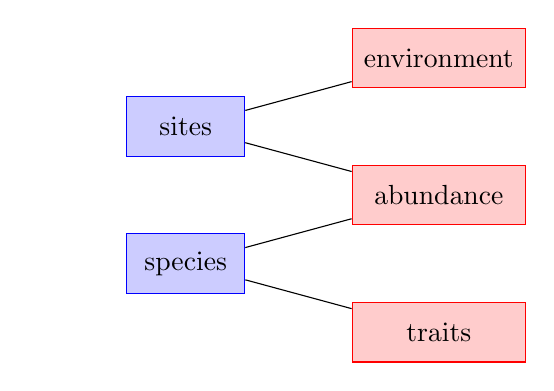
\begin{tikzpicture} [
	text centered,
	node distance=0.1cm,
	ndims/.style={
		rectangle,minimum width=1.5cm,draw=blue!=0,
		fill=blue!20
	},
	nvars/.style={
		rectangle,minimum width=2.2cm,draw=red!=0,
		fill=red!20
	},
	nblank/.style={
		rectangle,draw=red!=0,fill=red!0,draw opacity=0,
		minimum width=4cm
	}
]
\node [place,nblank]	(asites)					{};
\node [place,ndims]	(sites)[below=of asites]		{sites};
\node [place,nblank]	(bsites)[below=of sites]		{};
\node [place,ndims]	(species)[below=of bsites]		{species};
\node [place,nblank]	(bspecies)[below=of species]	{};
\node [place,nvars]	(environment)[right=of asites]	{environment}
	edge [-]		(sites);
\node [place,nvars]	(abundance)[right=of bsites]	{abundance}
	edge [-]		(sites)
	edge [-]		(species);
\node [place,nvars]	(traits)[right=of bspecies]		{traits}
	edge [-]		(species);
\end{tikzpicture}
\caption{Bipartite graph of the multiple-table structure of data with a standard fourth-corner problem (Fig. \ref{fig:fourth}).  Dimensions of replication are in blue and tables are in red.}
\label{fig:bipartite}
\end{figure}

To create a data list out of these data frames we use the \code{dcast} function, which was inspired by the \code{acast} function in the \code{reshape2} package \citep{Wickham2007}.
\begin{Schunk}
\begin{Sinput}
> dl <- dlcast(list(abundance,environment,trait),
 	dimids=c("sites","species"),
 	fill=c(0,NA,NA)
 )
> dl
\end{Sinput}
\begin{Soutput}
abundance:
---------
            capybara moss vampire
midlatitude        4    6       0
subtropical       10    0       1
tropical           8    9       0
equatorial         7    3       0
arctic             0    5       0
subarctic          0    0       0
Replicated along:  || sites || species || 


temperature:
-----------
midlatitude subtropical    tropical  equatorial      arctic 
         10          20          50          30          NA 
  subarctic 
          0 
Replicated along:  || sites || 


precipitation:
-------------
midlatitude subtropical    tropical  equatorial      arctic 
         20         100         150         200          NA 
  subarctic 
         40 
Replicated along:  || sites || 


body.size:
---------
capybara     moss  vampire 
     140        5      190 
Replicated along:  || species || 


metabolic.rate:
--------------
capybara     moss  vampire 
      20        5        0 
Replicated along:  || species || 


REPLICATION DIMENSIONS: 
  sites species 
      6       3 
\end{Soutput}
\end{Schunk}
This function takes three arguments:  (1) a list of data frames, (2) a character vector, \code{dimids}, with the names identifying the dimensions of replication (i.e. the names of the columns shared between the tables), and (3) a vector, \code{fill}, with one element for each data frame giving the value with which to fill in any structural missing values.  This last argument is particularly interesting, because we can fill missing abundances with zeros because those site-species combinations were not observed and \code{NA} values for the other tables.  This data list can now be used in analyses.

It is quite possible that your data are not stored in data frames with columns for both dimensions of replication and variables; this is not a large concern, as the \code{multitable} package offers many ways to get your data into a data list (see vignette ????).  However, we recommend that researchers at least consider what their data might look like in this format, because we believe that this format best illustrates concepts that will help make multiple-table data easier to understand, manage, and analyze.  I now finish with some further elaboration of these concepts.

\section{Multiple-table concepts}

Shared columns (i.e. dimensions of replication) between tables are expanded by \code{dlcast} into the dimensions of the arrays that are used to store each of the other columns (i.e. variables).  For example, because the \code{abundance} table has two dimensions of replication, it is stored as a two-dimensional matrix in the resulting data frame; whereas, the \code{environment} and \code{trait} tables have only two dimensions of replication and so are stored in one-dimensional vectors.

The benefits of the distinction between dimensions of replication and variables, is that it provides a common framework for understanding both simple and more complex multiple-table data structures.  In particular, the framework allows us to visualize the structure of complex data; for example the Lac Croche zooplankton community data (Fig. \ref{fig:beatrix}) has a structure given by Fig. \ref{fig:bipartitebeatrix}.  To store these data in a format amenable to \code{dlcast}, we would create one data frame for each of the groups of variables (red boxes) and add a column for each dimension of replication (blue boxes) associated with those variables.

\begin{figure}
\begin{tikzpicture} [
	text centered,
	node distance=0.1cm,
	ndims/.style={
		rectangle,minimum width=1.5cm,draw=blue!=0,
		fill=blue!20
	},
	nvars/.style={
		rectangle,minimum width=2.2cm,draw=red!=0,
		fill=red!20
	},
	nblank/.style={
		rectangle,draw=red!=0,fill=red!0,draw opacity=0,
		minimum width=4cm
	}
]
\node [place,nblank]	(abasin)					{};
\node [place,ndims]	(basin)[below=of abasin]		{basin};
\node [place,nblank]	(bbasin)[below=of basin]		{};
\node [place,ndims]	(time)[below=of bbasin]		{time};
\node [place,nblank]	(btime)[below=of time]		{};
\node [place,ndims]	(species)[below=of btime]		{species};
\node [place,nblank]	(bspecies)[below=of species]	{};
\node [place,nvars]	(environment)[right=of asites]	{environment}
	edge [-]		(basin)
	edge [-]		(time);
\node [place,nvars]	(abundance)[right=of bsites]	{abundance}
	edge [-]		(basin)
	edge [-]		(time)
	edge [-]		(species);
\node [place,nvars]	(scales)[right=of btime]		{time scales}
	edge [-]		(time);
\node [place,nvars]	(traits)[right=of bspecies]		{traits}
	edge [-]		(species);
\end{tikzpicture}
\caption{Bipartite graph of the Lac Croche data in Fig. \ref{fig:beatrix}.} 
\label{fig:bipartitebeatrix}
\end{figure}

With our data in this form, we can easily state the two requirements for using \code{data.list} objects:  (1) every table must share at least one dimension of replication with at least one other table and (2) at least one table must be replicated along all of the dimensions present in the data set.  The first criterion ensures that the tables will relate to each other; the second criterion ensures that some variables will be relatable to all other variables, a property that we feel is necessary for a response variable.  We also see that we only need more than one table if some variables are not replicated along all of the dimensions.

\section{Conclusion}

The structure of \code{data.list} objects is sufficiently rich to give rise to a much wider variety of uses than I could cover here.  However, this vignette was only intended to illustrate the basic features and concepts of the \code{multitable} package, and to justify its utility.  My long-term goal with the \code{multitable} project in general is to make standard analyses in \R\ (and beyond?) simpler to conduct on complex multiple-table data.

\section*{Acknowledgements}
I thank Guillaume Gu\'{e}nard, Levi Waldron, Ben Bolker, and Philip Dixon for discussions and suggestions about software design.

\bibliographystyle{plain}
\bibliography{Bibliography}

\end{document}
